\chapter{Einführung}

Unter den 20 häufigsten Todesursachen weltweit sind drei Krebsarten vertreten, eine davon ist Darmkrebs~\cite{Lozano.2012}.
Diese Krebsart hat die vierthöchste Sterblichkeitsrate von allen Krebsarten~\cite{Ferlay.2012}.
Polypen in der Darmschleimhaut bilden dessen Vorstufe~\cite{Kumar.2005}.

Regelmäßige Vorsorgeuntersuchungen ermöglichen es, das Wachstum solcher Kolorektalpolypen zu überwachen.
Hierbei wird in der Regel der Dickdarm im Rahmen einer Koloskopie endoskopisch untersucht~\cite{Kumar.2005} und von verdächtigen Polypen wird eine Gewebeprobe genommen, um diese anschließend histologisch auf ihre Gut- oder Bösartigkeit zu untersuchen.

Bei solchen Darmspiegelungen werden oftmals bis zu 28~\% aller Polypen übersehen~\cite{Leufkens.2012}.
Mit einer Markierung im endoskopischen Bild wie in \autoref{fig:highlight} könnte man Ärzten das Auffinden von Polypen erleichtern und die Fehlerrate verringern.
Grundlage dafür wäre eine automatische Lokalisierung von Polypen im koloskopischen Bild (s. \autoref{fig:segm}).

\begin{figure}[ht]
	\begin{subfigure}{.3\textwidth}
		\centering
		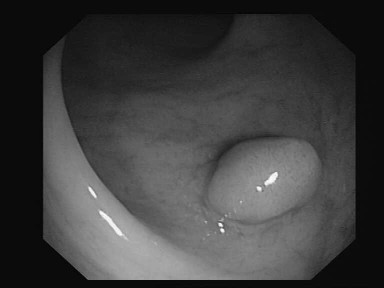
\includegraphics[width=.8\linewidth]{polyp129}
		\caption{}
		\label{fig:polyp}
	\end{subfigure}
	\begin{subfigure}{.3\textwidth}
		\centering
		
\includegraphics[width=.8\linewidth]{segm129}
		\caption{}
		\label{fig:segm}
	\end{subfigure}
	\begin{subfigure}{.3\textwidth}
		\centering
		% TODO Create graphic
		
\includegraphics[width=.8\linewidth]{segm129}
		\caption{}
		\label{fig:highlight}
	\end{subfigure}
	\caption{Kolorektalpolyp, dessen Segmentierung und Hervorhebung im Bild}
	\label{fig:polypseg}
\end{figure}

In der vorliegenden Masterarbeit wird zur Lösung dieses Lokalisierungsproblems ein Deep-Learning-Ansatz verwendet, der bisher noch nicht bei der Lokalisierung von Polypen eingesetzt wurde.
Dieser Ansatz, die \glspl{can} \cite{Isola.2017}, basiert auf den \glspl{gan} \cite{Goodfellow.2014}.

Dieses Kapitel erläutert die Problemstellung und stellt den Stand der Technik vor.
In den anschließenden Kapiteln erfolgt eine methodische Aufschlüsselung des Vorgehens in dieser Arbeit, die Umsetzung dieser Methodik, deren Ergebnisse und eine Analyse dieser Ergebnisse.




\section{Medizinische Grundlagen}

% polyps -> u. a. adenomas, fast nur diese werden bösartig
% je größer, desto höher wsk. bösartig



\section{Problemstellung und Motivation}





\section{Manuelle Feature Selection}\label{sec:manuelle-feature-selection}



\subsection{Lokalisierung}



\subsection{Segmentierung}





\section{Deep Learning}\label{sec:deep-learning}



\subsection{Convolutional Neural Networks}



\subsection{Lokalisierung}



\subsection{Segmentierung}



\subsection{Generative Netze}





\section{Fazit}


